% http://tex.stackexchange.com/questions/175671/how-to-use-arara-with-texshop
% !TEX TS-program = arara
% arara: xelatex
% arara: biber
% arara: nomencl
% arara: xelatex: { synctex: yes }
% arara: indent: { overwrite: yes, trace: yes  }
% arara: clean: {files: [IDAM-theory.aux, IDAM-theory.idx, IDAM-theory.ilg, IDAM-theory.ind, IDAM-theory.log, IDAM-theory.bbl, IDAM-theory.bcf, IDAM-theory.ist, IDAM-theory.blg, IDAM-theory.run.xml, IDAM-theory.nlo, IDAM-theory.nls]}

\documentclass[12pt]{article}


\usepackage[a4paper, top=1in, bottom=1.25in, left=1in, right=1in]{geometry}

\usepackage{amssymb,amsmath}
\usepackage{upgreek} % upright greek symbols

% xetex 西文字体
% https://www.reddit.com/r/typography/comments/2vzkad/a_good_serif_webfont_to_pair_with_fira_sans_thats/
\usepackage{fontspec,xltxtra,xunicode}
    \setmainfont[BoldFont={Charter Bold}, ItalicFont={Charter Italic}]{Charter}
    \setmonofont{Fira Mono}

% 中文字体
\usepackage{xeCJK}
    \setCJKmainfont[BoldFont={Songti SC Bold}, ItalicFont={Kaiti SC Regular}]{Songti SC Regular}
    \xeCJKsetup{CJKecglue = {\hskip 0pt plus 0.08\baselineskip}, xCJKecglue = {false}}
    \punctstyle{plain}

% don't move this line above
\defaultfontfeatures{Mapping=tex-text,Scale=MatchLowercase}

% Line spacing
\linespread{1.5}

% use upquote if available, for straight quotes in verbatim environments
\IfFileExists{upquote.sty}{\usepackage{upquote}}{}
% use microtype if available
\IfFileExists{microtype.sty}{%
    \usepackage{microtype}
    \UseMicrotypeSet[protrusion]{basicmath} % disable protrusion for tt fonts
}{}

\usepackage[unicode=true]{hyperref}
    \urlstyle{same}  % don't use monospace font for urls

\usepackage{graphicx,grffile}
\makeatletter
\def\maxwidth{\ifdim\Gin@nat@width>\linewidth\linewidth\else\Gin@nat@width\fi}
\def\maxheight{\ifdim\Gin@nat@height>\textheight\textheight\else\Gin@nat@height\fi}
\makeatother
% Scale images if necessary, so that they will not overflow the page
% margins by default, and it is still possible to overwrite the defaults
% using explicit options in \includegraphics[width, height, ...]{}
\setkeys{Gin}{width=\maxwidth,height=\maxheight,keepaspectratio}
\IfFileExists{parskip.sty}{%
\usepackage{parskip}
}{% else
\setlength{\parindent}{0pt}
\setlength{\parskip}{6pt plus 2pt minus 1pt}
}
\setlength{\emergencystretch}{3em}  % prevent overfull lines
\providecommand{\tightlist}{%
    \setlength{\itemsep}{0pt}\setlength{\parskip}{0pt}}
\setcounter{secnumdepth}{0}
% Redefines (sub)paragraphs to behave more like sections
\ifx\paragraph\undefined\else
\let\oldparagraph\paragraph
\renewcommand{\paragraph}[1]{\oldparagraph{#1}\mbox{}}
\fi
\ifx\subparagraph\undefined\else
\let\oldsubparagraph\subparagraph
\renewcommand{\subparagraph}[1]{\oldsubparagraph{#1}\mbox{}}
\fi

% set default figure placement to htbp
\makeatletter
\def\fps@figure{htbp}
\makeatother

%%% custom settings

% subcaption
% http://tex.stackexchange.com/questions/125579/subcaption-with-beamer
\usepackage[compatibility=false]{caption}
\usepackage{subcaption}

% for gif
\usepackage{animate}

% chemistry
\usepackage[version=3]{mhchem}
% make inline codes smaller
%\renewenvironment{texttt}{\small}{}
\renewcommand{\texttt}[1]{{\small\ttfamily #1}}

\usepackage{nomencl}
\makenomenclature

\usepackage{etoolbox}


\title{估算群体中的 indel 附近 \\ 单核苷酸突变率相对增加的模型}
\date{\vspace{-5ex}}

%%% document starts here

\begin{document}

\maketitle

假设 indel 的发生率 $\mu_\text{i}$ 很小, 并且是中性的.
对于 indel 和 nonindel 等位基因, 令 $\mu$ 和 $\mu_\text{het}$ 分别代表纯合子和杂合子中的中性核苷酸突变,
并且令 $f = \mu_\text{het} / \mu$.
指定 $N_\text{i}$ 和 $N_\text{ni}$ 分别代表 indel 和 nonindel 附近自 MRCA 之后的中性突变数.
我们要寻求期望值 $E(N_\text{i})$ 和 $E(N_\text{ni})$.

\begin{figure}
    \centering
    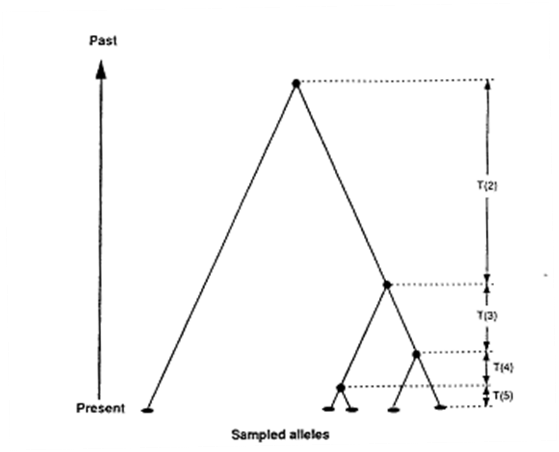
\includegraphics[width=8cm]{IDAM-theory.images/image1.png}
    \caption{
        $n$ 个基因的样本中 $k$ 个基因含有中性 indel $I$ 的中性系谱.
        回溯到 $I$ 的时间为 $T$, $T^*$ 代表回溯到样本共同祖先 MRCA 的额外的时间.
        $I$ 处的世系数为 $\nu$.
    }
    \label{fig:1}
\end{figure}

在图 \ref{fig:1} 的系谱中, $n$ 个基因的样本中 $k$ 个携带 indel,
由 $k \geq 1$ 且 $n-k \geq 1$, 可知 $1 \leq k \leq n-1$;
$I$ 处的世系数为 $\nu$, 由 $\nu \geq 2$ 且 $n-k \geq \nu - 1$, 可知 $2 \leq \nu \leq n-k+1$.
以 $2N_\text{e}$ 个世代为单位衡量所有时间, 其中 $N_\text{e}$ 代表有效群体大小.
回溯到 $I$ 的时间是 $T$, $T^*$ 代表回溯到样本共同祖先 MRCA 的额外的时间.
忽略 $k$ 和 $n$ 的相关性.

根据标准的中性突变模型 (Kimura 1983;Watterson 1975)有:
\begin{equation} \label{eq:1}
    E(S) = \mu E(T_{\text{tot}})
    \text{.}
\end{equation}

这个模型的基本假设是:
\begin{itemize}[leftmargin=4em]
    \item 每个子代相对于亲代的突变个数服从泊松分布, 平均值为 $\mu$;
    \item $\mu$ 为常数, 与群体大小、基因型和时间无关;
    \item 无选择和重组.
\end{itemize}

对于一个 indel, $T_\text{het}$ 和 $T_\text{hom}$ 分别代表 indel 在杂合子和纯合子中经历的时间. 可知:
\begin{equation} \label{eq:2}
    T = T_\text{het} + T_\text{hom}
    \text{,}
\end{equation}
根据方程 \ref{eq:1} 和 \ref{eq:2} 可以得到 $E(N_\text{i})$:
\begin{equation} \label{eq:3}
    \begin{split}
        E(N_\text{i})
        &= 2 N_\text{e} [\mu_\text{het}E(T_{\text{het}}) + \mu E(T_{\text{hom}}) + \mu E(T^*)] \\
        &= 2 N_\text{e}\mu [\frac{\mu_\text{het}}{\mu} E(T_{\text{het}}) + E(T_{\text{hom}}) + E(T^*)] \\
        &= \frac{\theta}{2} [f E(T_{\text{het}}) + E(T_{\text{hom}}) + E(T^*)] \\
        &= \frac{\theta}{2} [f E(T_{\text{het}}) + f E(T_{\text{hom}}) - f E(T_{\text{hom}}) + E(T_{\text{hom}}) + E(T^*)] \\
        &= \frac{\theta}{2} [f E(T) + E(T^*) - (f - 1) E(T_{\text{hom}})]
        \text{,}
    \end{split}
\end{equation}
其中 $\theta = 4N_\text{e}\mu$.

在过去的 $t$ 时刻, indel 的频率是 $X(t)$, 则:
\begin{itemize}[leftmargin=4em]
    \item indel 在杂合子中的条件概率为 $1-X(t)$;
    \item indel 在纯合子中的条件概率为 $X(t)$;
    \item  nonindel 在杂合子中的条件概率为 $X(t)$;
    \item  nonindel 在纯合子中的条件概率为 $1-X(t)$.
\end{itemize}
在 $t$ 时刻 indel 纯合性的指示函数为:
\begin{equation} \label{eq:4}
    \chi_\text{hom}(t) =
    {\begin{cases}
        1 & \text{如果 indel 在时刻~} t \text{~处于纯合子}, \\
        0 & \text{如果 indel 在时刻~} t \text{~处于杂合子}.
        \end{cases}}
\end{equation}
因此,
\begin{equation} \label{eq:5}
    T_\text{hom} = \int_{0}^{T} \chi_\text{hom}(t)dt \text{.}
\end{equation}
这导出了条件期望
\begin{equation} \label{eq:6}
    \begin{split}
        E[T_\text{hom} | X(0)=x]
        &= E \left\{ E\left[ \int_{0}^{T} \chi_\text{hom}(t) dt \mathrel{\Big|} T, X(0)=x  \right] \right\} \\
        &= E \left\{ \int_{0}^{T} E[\chi_\text{hom}(t)] dt \mathrel{\Big|} X(0)=x \right\} \\
        &= E \left\{ \int_{0}^{T} X(t) dt \mathrel{\Big|} X(0)=x \right\}
        \text{.}
    \end{split}
\end{equation}
类似地, 可得
\begin{equation} \label{eq:7}
    E[T_\text{het} | X(0)=x] = E \left\{ \int_{0}^{T} [1-X(t)] dt \mathrel{\Big|} X(0)=x \right\}
    \text{.}
\end{equation}

交换 $E[T_\text{het}]$ 和 $E[T_\text{hom}]$, 用上一段的推导方法可得
\begin{equation} \label{eq:8}
    \begin{split}
        E(N_\text{ni})
        &= \frac{\theta}{2} [f E(T_{\text{hom}}) + E(T_{\text{het}}) + E(T^*)] \\
        &= \frac{\theta}{2} [E(T) + E(T^*) + (f - 1) E(T_{\text{hom}})]
        \text{.}
    \end{split}
\end{equation}
这样, 我们必须计算方程 \ref{eq:3} 和 \ref{eq:8} 里的三个平均时间.
自此以后, 假设 $\theta_\text{i} = 4N_\text{e}\mu_\text{i} \rightarrow 0$,
并忽略 indel 到 nonindel 的回复突变.

为了计算方程 \ref{eq:6}, 首先要注意 indel 在群体中还没有固定 ($0 \le k \le n$),
可用 \textcite{maruyama1975} 的方程 16 来计算一个 indel 固定前的平均时间:
\begin{equation*}
    \lim_{p \to 0} \frac{F_x^\text{(1)}(p)}{\Phi(p, x)}
    = \frac{4N_\text{e}}{1-4N_\text{e}\nu}
    \left\{
    \int_0^x \frac{1-(1-\xi)^{1-4N_\text{e}\nu}}{\xi} d\xi \\
    + \frac{1-(1-x)^{1-4N_\text{e}\nu}}{(1-x)^{1-4N_\text{e}\nu}}
    \int_x^1 \frac{(1-\xi)^{1-4N_\text{e}\nu}}{\xi} d\xi
    \right\}
    \text{.}
\end{equation*}
根据我们的需要对这个方程做修改:
(i) 除以 $2N_\text{e}$ 来衡量时间;
(ii) 突变率趋近于 0, 即 $4N_\text{e}\nu$ 趋近于 0;
(iii) 在两个被积函数中都插入一个因子 $\xi$, 即同乘以 $\xi$. 可以得到:
\begin{equation} \label{eq:9}
    \begin{split}
        E[T_\text{hom} | X(0)=x]
        &= 2 \int_0^x \xi d\xi + \frac{2x}{1-x} \int_x^1 (1-\xi) d\xi \\
        &= x^2 + \frac{2x}{1-x} \left(\frac{1}{2} (x - 1)^2 \right) \\
        &= x
        \text{.}
    \end{split}
\end{equation}

为了从方程 \ref{eq:9} 中推导出 $E[T_\text{hom}]$, 需要得到在 $n$ 个基因的样本中观察到 $k$ 个 indels 的概率密度 $X(0)$.
根据贝叶斯公式,群体频谱为 $\theta/x$ \parencite{kimura1969, kimura1971a, ewens2004},
样本频谱为 $\theta_\text{i}/x$ \parencite{watterson1975, ewens2004}, 可以得条件密度为
\begin{equation} \label{eq:10}
    \begin{split}
        \phi(x)
        &= \binom{n}{k} x^k (1-x)^{n-k} \frac{\theta_\text{i}}{x} / \frac{\theta_\text{i}}{k} \\
        &= k \binom{n}{k} x^{k-1} (1-x)^{n-k}
        \text{.}
    \end{split}
\end{equation}
结合方程 \ref{eq:9} 和 \ref{eq:10} 得到
\begin{equation} \label{eq:11}
    a \equiv E(T_\text{hom}) = \frac{k}{n+1}
    \text{.}
\end{equation}

从 \textcite{wiuf1999} 得知:
\begin{equation} \label{eq:12}
    b \equiv E(T) = \frac{2k}{n-1} - \frac{2}{n}
    + 2 \binom{n-1}{k}^{-1} \sum_{j=2}^{n-k+1} \frac{1}{j} \binom{n-j-1}{k-1}
    \text{.}
\end{equation}

\newpage
\renewcommand{\nomname}{} % no nomenclature title

% nomenclature groups
\renewcommand\nomgroup[1]{%
    \item[\large\bfseries
        \ifstrequal{#1}{A}{缩写}{%
            \ifstrequal{#1}{B}{符号}{%
                \ifstrequal{#1}{C}{函数}{%
                    \ifstrequal{#1}{N}{名词}{%
                        \ifstrequal{#1}{P}{短语}{%
        }}}}}%
    ]
}

\nomenclature[A, 01]{DNA}{Deoxyribonucleic acid, 脱氧核糖核酸}
\nomenclature[A, 02]{MRCA}{Most Recent Common Ancestor, 最近共同祖先}
\nomenclature[A, 03]{Indel}{Insertion/Deletion, 插入/缺失}

\nomenclature[B, 01]{$\mu$}{The mean number of mutations, 突变数的平均值}
\nomenclature[B, 02]{$t$}{The number of generations since the MRCA of two sampled homologous sequences, 从 MRCA 到两个抽样的同源序列的世代数}
\nomenclature[B, 03]{$S$}{The number of mutations that have occurred in the descent to the two descendent sequences, 向下到这两个后代的序列过程中产生的突变数}
\nomenclature[B, 04]{$T_{\text{tot}}$}{The sum of the lengths of the branches of the genealogy of a sample, 一个样本的系谱中所有分支长度的总和}

\nomenclature[C, 01]{$E()$}{Expected value, 期望值}
\nomenclature[C, 02]{$\text{Var}()$}{Variance of expected value, 期望值的方差}

\nomenclature[N]{Patterns}{样式}
\nomenclature[N]{Pedigree}{家谱}
\nomenclature[N]{Lineage}{世系}
\nomenclature[N]{Genealogy}{系谱}
\nomenclature[N]{Sample}{样本}
\nomenclature[N]{Sampling}{抽样}
\nomenclature[N]{Gene tree}{基因树}
\nomenclature[N]{Forces}{力量}
\nomenclature[N]{Polymorphism}{多态性}
\nomenclature[N]{Homologous sequences}{同源序列}
\nomenclature[N]{Coalescent process}{溯祖过程}
\nomenclature[N]{Alleles}{等位基因}
\nomenclature[N]{Mutations}{突变}
\nomenclature[N]{Segregating sites}{隔离位点}
\nomenclature[N]{Variations}{变异}
\nomenclature[N]{Equation}{方程}
\nomenclature[N]{Demographics}{人口统计学}
\nomenclature[N]{Fitness}{适合度}
\nomenclature[N]{Sampled allele}{样本等位基因}
\nomenclature[N]{Stochastic precess}{随机过程}
\nomenclature[N]{Restriction map}{限制性图谱}
\nomenclature[N]{Moment generating function}{矩母函数}
\nomenclature[N]{Hitchhiking}{搭乘效应}
\nomenclature[N]{Distritution}{分布}

\nomenclature[N]{Indicator function}{指示函数}
\nomenclature[N]{Homozygote}{纯合子}
\nomenclature[N]{Heterozygote}{杂合子}
\nomenclature[N]{Conditional expectation}{条件期望}
\nomenclature[N]{Probability density}{概率密度}
\nomenclature[N]{Bayes' formula}{贝叶斯公式}
\nomenclature[N]{Frequency spectrum}{频谱}

\nomenclature[P, 01]{Properties of genealogy}{系谱特性}
\nomenclature[P, 02]{Statistical properties of genealogy}{系谱的统计特性}
\nomenclature[P, 03]{The sampling that produces one generation from the last}{上一代形成下一代的模式, 代间模式}
\nomenclature[P, 04]{Samples of allele}{等位基因样本}
\nomenclature[P, 05]{Bear, bearing, bore}{携带}
\nomenclature[P, 05]{Selectively maintained}{选择性保留地}
\nomenclature[P, 06]{Infinite-sites model}{无限位点模型}
\nomenclature[P, 07]{Infinite allele model}{无限等位基因模型}

\printnomenclature

\newpage
\section*{参考文献}
\addcontentsline{toc}{section}{参考文献}

\printbibliography[heading=none]

\end{document}
